\chapter{Preparation of Datasets}
\label{chap:preparations data sets}
% Todo: 6 pages?

Next to the ML model selected, the data used to train and evaluate the model has a major influence on its performance. If the data is not representative of the underlying process that the model should be fitted to, there can be bias or an inability to generalize well to new data. In this chapter, we take a look at potential data sources and discuss the construction process of the datasets used in this work.\\
In the field of natural language processing (NPL) and computer vision (CV), there is an abundance of large available datasets which have a big contribution to the advancements in the field, e.g. annotated datasets as provided by Google Research~\footnote{\url{https://research.google/resources/datasets/}}. In the field of climate research, there are also many datasets, including satellite data, weather station data, and climate model data. For the specific use case of temperature interpolation in urban areas, an optimal dataset would contain high spatial and temporal resolution sensor data, e.g. a high sensor density and a low time interval of f.e. five to ten minutes. Additionally, the sensor placement and sensor quality have a high influence on the accuracy of the sensor readings, as discussed in~\ref{subsec: Sensing Layer}, therefore the correct placement and calibration of the sensors needs to be guaranteed. Such requirements are not met by traditional weather station networks as the spatial coverage is too low, as seen in figure~\ref{fig:dwd sensor locations germany} which shows the weather station network of the official german weather services (DWD).
However, they are met by dense sensor networks. A mayor challenge of running such a dense sensor network in a controlled scientific environment is the potential high cost of individual sensors, e.g. high precision and calibration, and the maintenance of the network, e.g. battery replacement, damages due to environmental influences, theft etc. 
There are several projects that run climate dense sensor networks~\cite{muller2013sensors}. %TODO: incoporate this into the text


Therefore, there are very few such projects and currently no openly available datasets. There were projects in the past such as the Helsinki Testbed~\cite{koskinen2011helsinki} or the Birmingham Urban Climate Laboratory~\cite{warren2016birmingham}, but links to their datasets are unfortunately not maintained, showing the difficulty of finding and retrieving relevant datasets in this field.\\
As an alternative, in this work we instead mainly use data from citizen run sensor networks, e.g. crowdsourced data from personal weather stations (PWS), also called citizen weather stations (CWS), which are either openly available or can be requested in limited fashion via provided APIs. In this work we create train and test datasets by combining openly available sensor data from the providers Sensor Community, Netatmo, and the official german weather services (DWD) for quality control. Other sources for crowdsourced weather station data include WeatherObservationsWebsite (WOW)~\footnote{\url{https://wow.metoffice.gov.uk/}} and Weather Underground~\footnote{\url{https://www.wunderground.com/}}. WOW is a platform run by the UK Met Office, which is the UK's national weather service, and has a dense sensor coverage in the UK and the Netherlands as seen in figure \ref{fig:wow sensor locations}. Weather Underground is a commercial weather service which also provides a crowdsourced weather station network. Unfortunately, Weather Underground only provides an API for users with a registered weather station or other bulk download options for historical data. The website would allow for manual download of historical data, but this is not feasible for the amount of data needed for this work.
% TODO: talk about static data such as NDVI

\begin{figure}[ht]
    \centering
    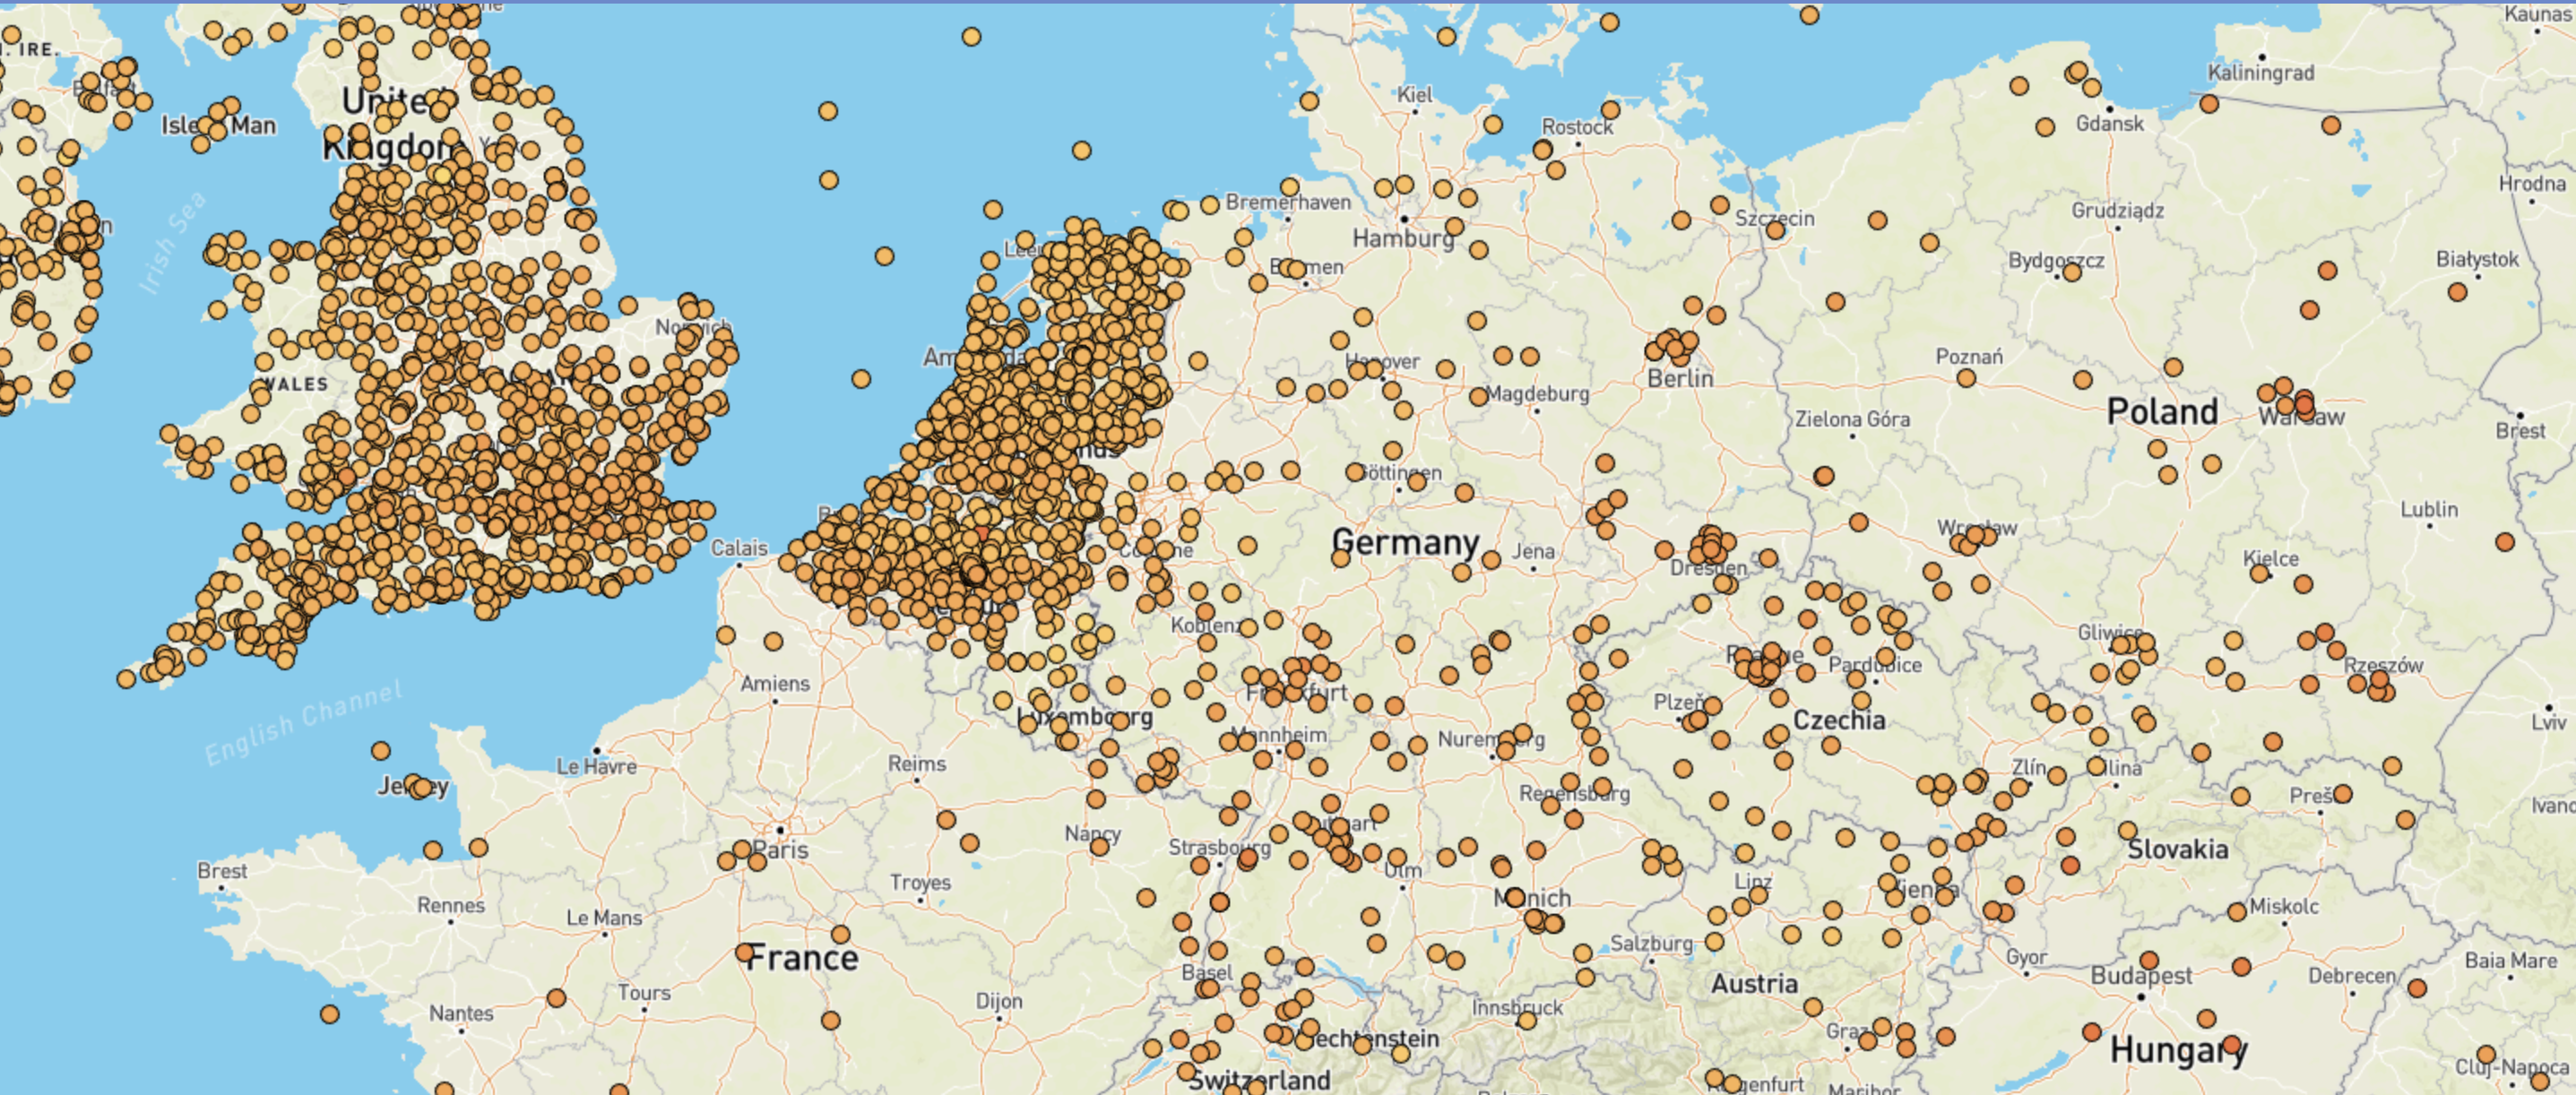
\includegraphics[width=1\textwidth]{images/wow_sensor_locations.png}
    \caption{Temperature sensor locations from WOW, acessed on 05.07.2023}
    \label{fig:wow sensor locations}
\end{figure}

\section{Sensor Community}

Sensor Community~\footnote{\url{https://sensor.community/en/}} is a contributers driven global sensor community that creates Open Environmental Data, and has an archive available~\footnote{\url{https://archive.sensor.community/}} of their historical sensor data world wide. There are no quality measures recorded for each sensor, but as crowd-sourced sensor data tends to have a lower quality than professsionally setup sensors, e.g. sensor placement by non-professionals, we need to explore how the data quality looks like.
In Figure~\ref{fig:temperature_sensor_community_map}, where we see the greater Hamburg area with a currently reported temperature of 25°C by the DWD Fuhlsbüttel station, there are multiple sensors that report a temperature of 30°C and above, which could be either due to the sensor being placed in direct sunlight or due to the sensor being faulty. An outlier near Pinneberg is shown in fig.~\ref{fig:temperature_sensor_community_outlier}, where one sensor reports 25°C, as currently expected, and one sensor reporting 50°C, which is clearly an outlier. This data quality issue needs to be adressed in the data pre-processing step and can result in a significant reduction of available data. This was also an issue dicussed in~\cite{meier2017crowdsourcing}, as ``erroneous metadata, failure of data collection, and unsuitable exposure of sensors lead to a reduction of data availability by 53 \%``.

\begin{figure}[ht]
    \centering
    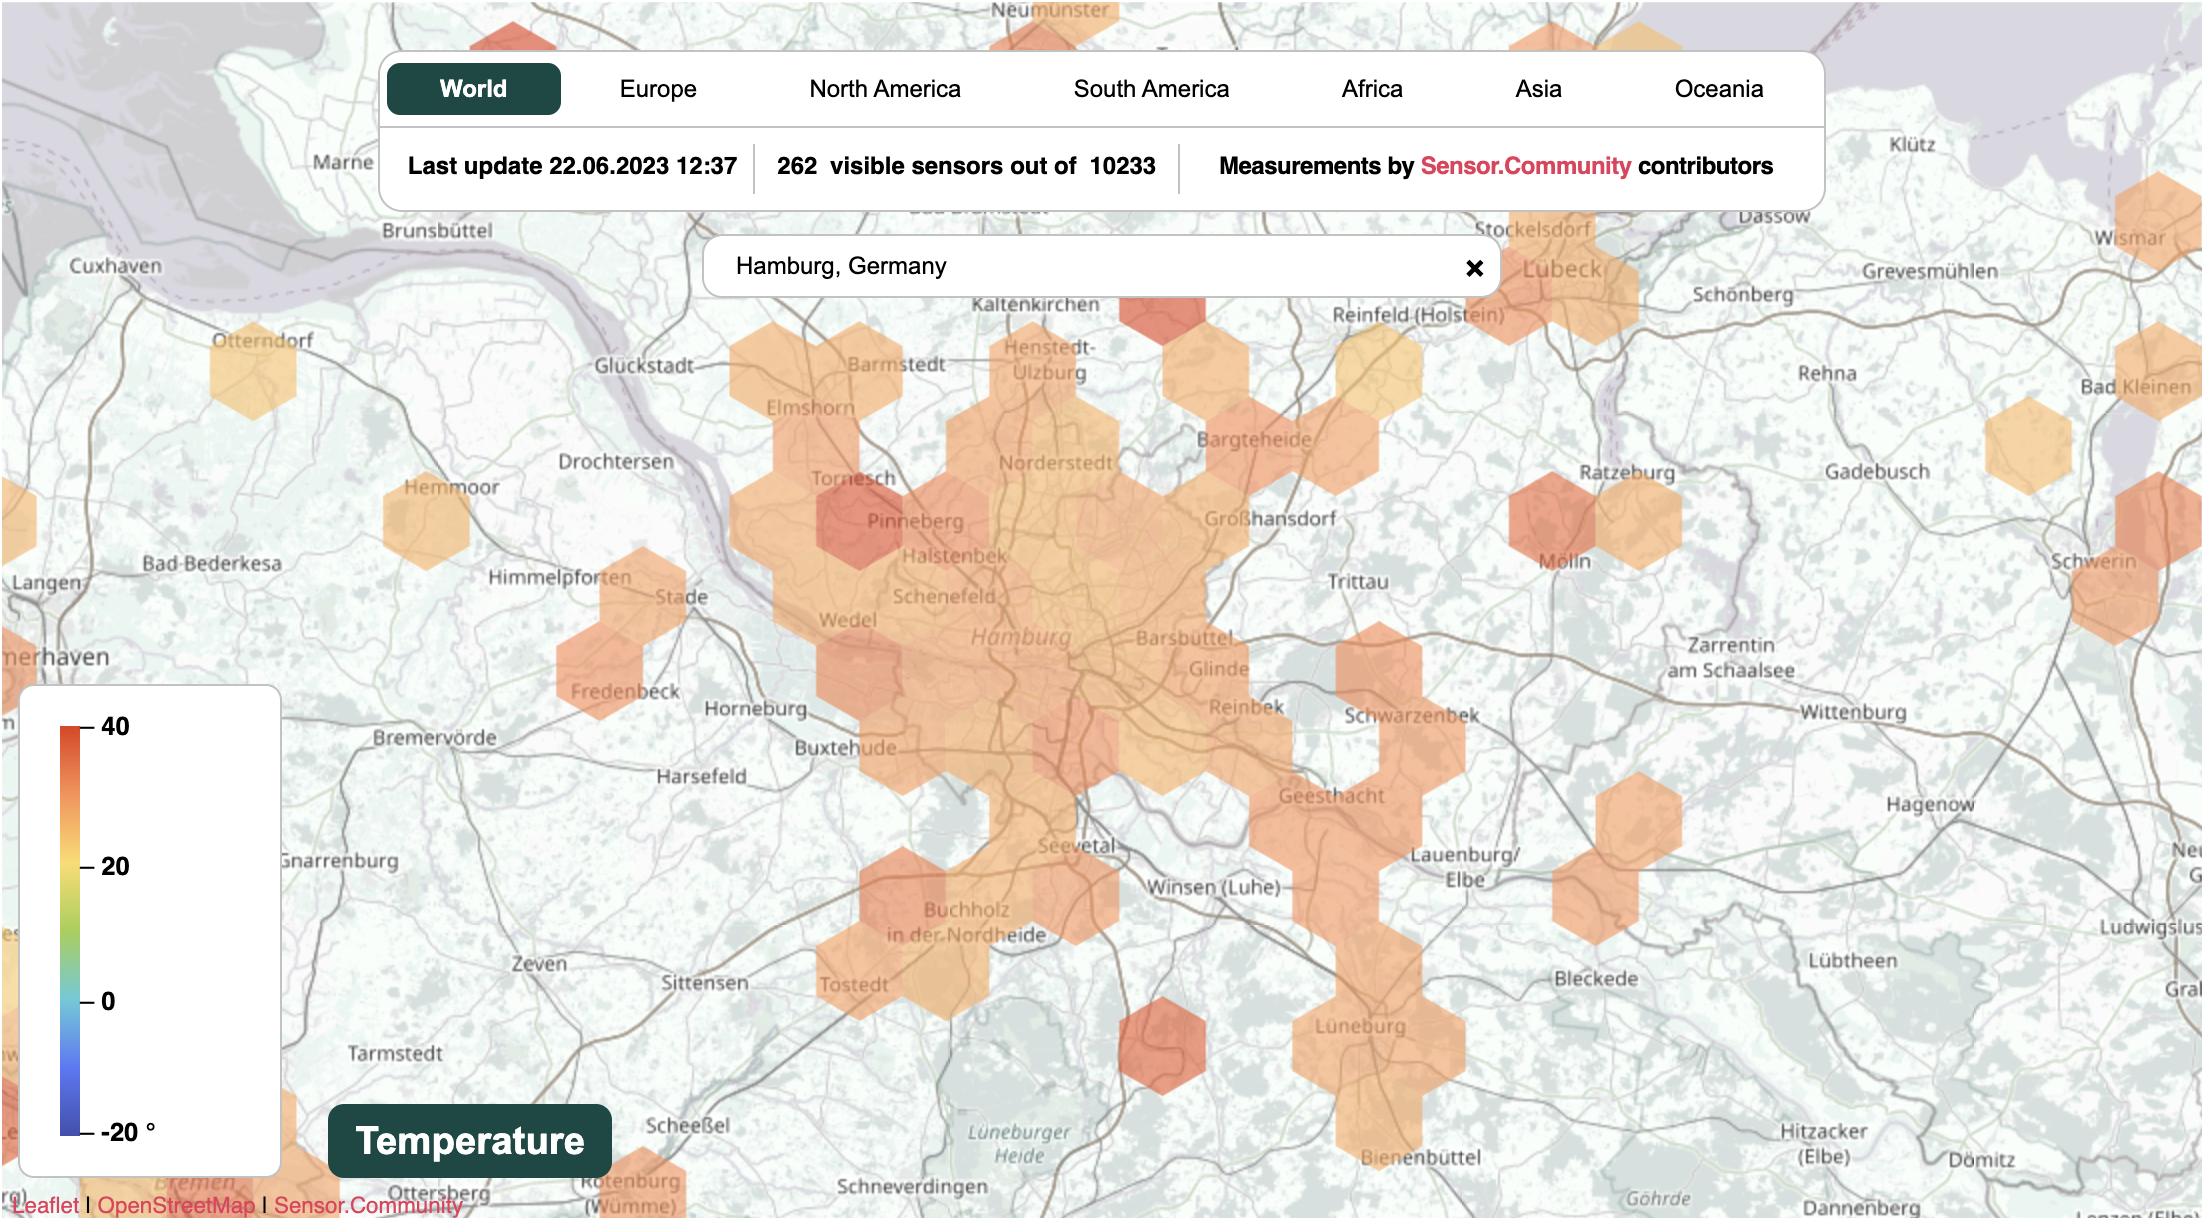
\includegraphics[width=1\textwidth]{images/sensor_community_temperature_map.png}
    \caption{Temperature map from Sensor Community for Hamburg, Germany, on 22.06.2023 12:51h with the DWD reference at 25°C}
    \label{fig:temperature_sensor_community_map}
\end{figure}

\begin{figure}[ht]
    \centering
    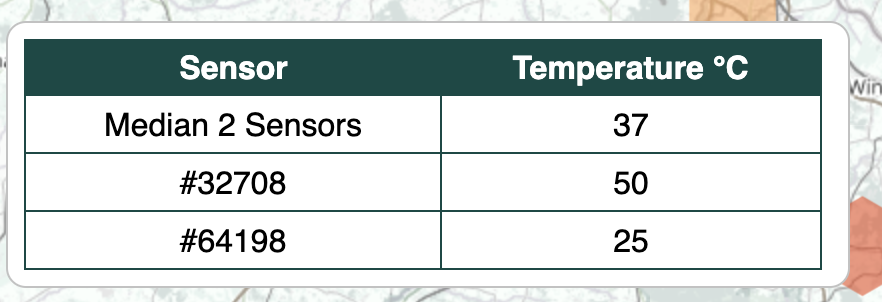
\includegraphics[width=0.8\textwidth]{images/sensor_community_outliers.png}
    \caption{Temperature outlier from Sensor Community for Hamburg, Germany, on 22.06.2023 12:51h with the DWD reference at 25°C}
    \label{fig:temperature_sensor_community_outlier}
\end{figure}

Overall, there are around 11.738 active sensors~\footnote{as of 24.06.2023}. Of these sensors, many are located in Germany and almost half of them are of type BME 280, which is a lost-cost Bosch sensor which can measure temperature, pressure and humidity, as seen in Appendix~\ref{sensor_community_sensors_by_countries}. The sensor locations as of may 2023 are shown in~\ref{fig:sensor community sensor locations germany}. DHT22 sensors can measure temperature and humidity, BMP280 and BMP180 sensors can measure temperature and pressure, and BME280 sensors can measure temperature, pressure and humidity.\\

\begin{figure}[ht]
    \centering
    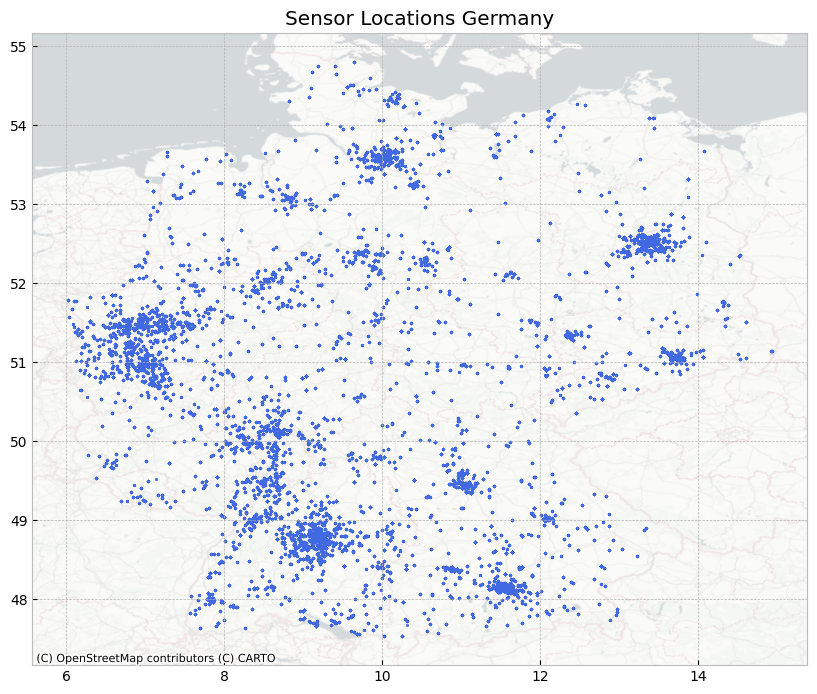
\includegraphics[width=1\textwidth]{images/sc_sensor_locations_germany.png}
    \caption{Sensor locations of Sensor Community in Germany, as of 01.05.2023, of sensor type DHT22 (2590 sensors), BME280 (1558 sensors), BMP280 (100 sensors), BMP180 (72 sensors)}
    \label{fig:sensor community sensor locations germany}
\end{figure}

\section{Netatmo}

Netatmo~\footnote{\url{https://www.netatmo.com/en-eu}} is an american company that sells smart-home devices including weather stations. They host a weather map~\footnote{\url{https://weathermap.netatmo.com/}} where customers can share their weather station data. The provide an API to access current weather station data. They provide historical and current weather data for commercial partners or partners in the research and education sector. They are part of the EUMETNET project~\footnote{\url{https://www.eumetnet.eu/}} which is a network of 31 European meteological and hydrological services (NMHSs). The project aims to facilitate the exchange of weather data and to improve the quality of weather forecasts, especially in the context of PWS~\cite{hahn2022observations}. There are currently no openly historical datasets available, only private datasets such as \url{https://catalogue.ceda.ac.uk/uuid/e8793d74a651426692faa100e3b2acd3} (last acessed 05.07.2023), that are only available for EUMETNET members. They offer an educational program~\footnote{\url{https://www.netatmo.com/en-eu/weather-with-netatmo}} to acess limited amounts of data that is usually only available to commercial partners.

\begin{figure}[ht]
    \centering
    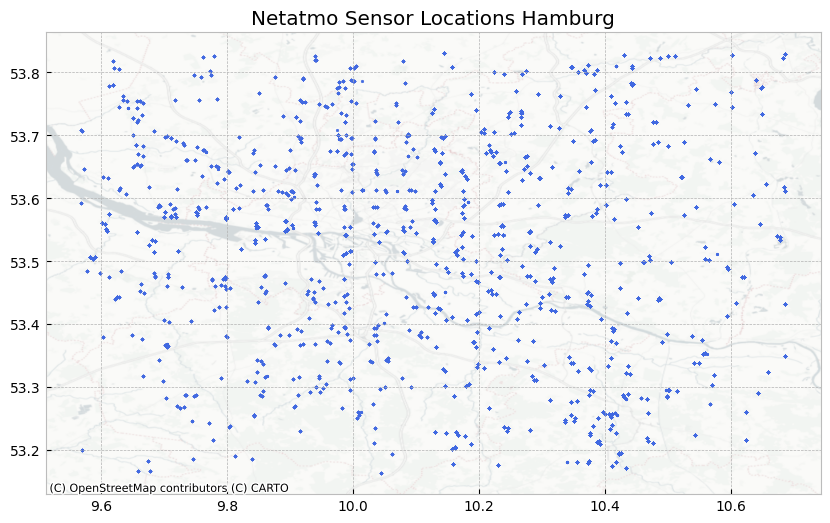
\includegraphics[width=1\textwidth]{images/netatmo_sensor_locations_germany.png}
    \caption{Sensor locations of Netatmo in Hamburg, Germany, as of 28.06.2023}
    \label{fig:netatmo sensor locations germany}
\end{figure}

In this work, data from Netatmo stations is primarily used as Netatmo offers a large amount of sensors in Germany, as seen in figure~\ref{fig:netatmo sensor locations germany}. Due to the limitations of the API rate limits, only data for the region of Hamburg, Germany is used.

% TODO: rewrite the following:

\textbf{Netatmo}: Netatmo~\footnote{\url{https://www.netatmo.com/}} is a French Smart Home Company that was founded in 2011. It has a large smart home assortment including cameras, door bells, smoke detectors, thermostats and weather stations among others. In the context of collecting meteological data, the smart weather products are of particular interest. These include a smart weather station that collects air temperature, humidity and air pressure, an anemometer that collects wind speed and direction, and a rain gauge. The sensor specifications, as reported by the vendor himself, is reported in Table \ref{tab: netatmo sensor specs}.\\
Complementary to its smart products, Netatmo also operates a weather platform and a developer portal. The weather platform offers a weather map~\footnote{\url{https://weathermap.netatmo.com/}} containing the measurements of connected weather stations accross the whole world for air temperature, precipitation, and wind speed and directon. The developer portal~\footnote{\url{https://dev.netatmo.com/apidocumentation}} offers a way to programmatically access all sensor measurements via a REST API. In this work, we later use this REST API to collect sensor data, as discussed in Chapter \ref{chap:preparations data sets}.

% precisions
% Please add the following required packages to your document preamble:
% \usepackage{booktabs}
\begin{table}[]
\begin{tabular}{@{}lllll@{}}
\toprule
Measurement    & Unit    & Measurement Range      & Precision  & Recording Frequency              \\ \midrule
Temperature    & °C      & -40°C to 65°C          & 0.3°C   & averaged over 5 min              \\
Humidity       & \% (RH) & 0 to 100\%             & 3\%     & -                                \\
Air Pressure   & mbar    & 260 to 1160 mbar       & 1mbar   & -                                \\
Noise          & dB      & 35 to 120 dB           & -       & -                                \\
Wind Speed     & m/s     & 0 to 45 m/s (160 km/h) & 0.5 m/s & every 6 sec, averaged over 5 min \\
Wind Direction & °       & 0 to 359°              & 5°      & every 6 sec, averaged over 5 min \\
Rainfall       & mm/h    & 0.2 to 150 mm/h        & 1mm/h   & every 5 min (bucket is emptied)  \\ \bottomrule
\end{tabular}
\caption{Netatmo Sensor Specifications (Vendor reported)}
\label{tab: netatmo sensor specs}
% todo: adjust to page size, maybe move to dataset chapter
\end{table}

\subsubsection{Quality Considerations}

Netatmo sensors have a good measurement accuracy, however due to the compact design, an aluminium housing, poor ventilation due to the small case, no dedicated radiation screen resultiing in a proneness to radiative errors, and therefore overall slow sensor-response time~\cite{meier2017crowdsourcing, buchau2018modelling}, Netatmo weather stations have a systematic bias that influences data quality. Due to the uniformity of Netatmo sensors, e.g.\ all sensors are build in the same way, this bias could be corrected in the QC step.

\section{DWD}

The official german weather service (DWD) has many objectives, that are defined by the DWD-law in Germany. Its tasks include meterological and climatological monitoring of the atmosphere, responsibility for meterologically securing airspace for civil aviation, monitoring the maritim climate and more. The DWD operates a large monitoring network and publishes most of it's data via its OpenData portal~\footnote{\url{https://opendata.dwd.de/}, last accessed 13.07.2023}.\\
The main advantages of the DWD data are high data quality through reference instruments and proper setup according to WHO guidelines~\cite{oke2006guideline}. The main disadvantage is the low spatial coverage of the data, as stations are sparsely distributed to measure the overall mesoscale climate, as seen in Figure~\ref{fig:dwd sensor locations germany}. Additionally, a lot of the public weather stations are located at airports, which are usually located outside of cities, and therefore not suitable for measuring urban microclimates.

\begin{figure}[ht]
    \centering
    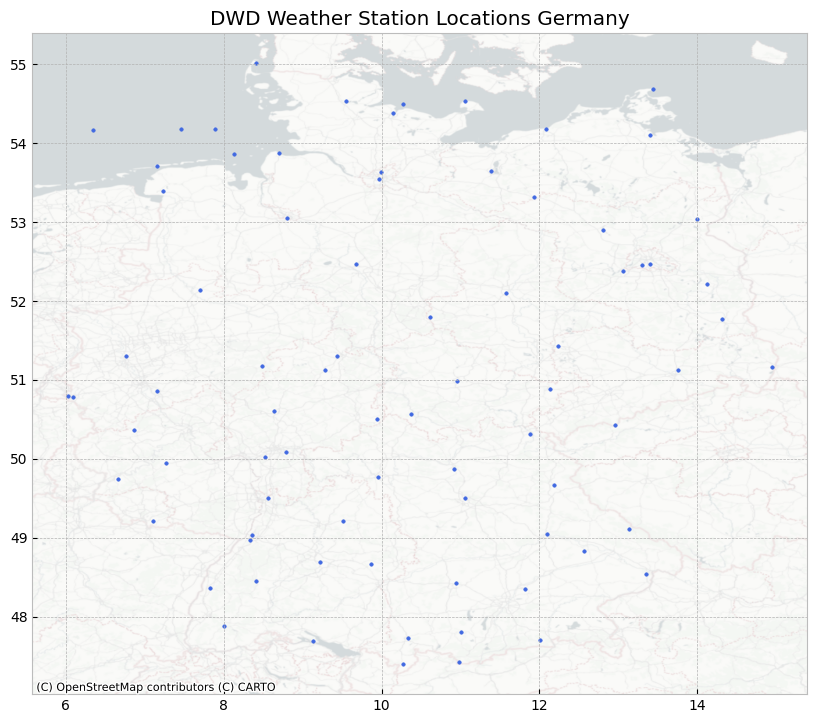
\includegraphics[width=1\textwidth]{images/dwd_weather_station_locations_germany.png}
    \caption{DWD Weather Station Locations in Germany, \url{https://opendata.dwd.de/climate_environment/CDC/observations_germany/climate/subdaily/standard_format/KL_Standardformate_Beschreibung_Stationen.txt}, accessed 28.06.2023}
    \label{fig:dwd sensor locations germany}
\end{figure}

\subsubsection{Urban Climate Stations}

Next to the official weather stations, the DWD also operates urban weather stations, however there are currently only four stations in the following cities:

\begin{itemize}
    \item Berlin-Alexanderplatz, Berlin, Berlin
    \item Freiburg-Mitte, Freiburg, Baden-Württemberg
    \item Hannover-Nordstadt, Hannover, Niedersachsen
    \item Dresden-Neustadt, Dresden, Sachsen
\end{itemize}

The number of urban weather stations is planned to be gradually extended to reach 10 stations with the locations being primarily determined by the measurement objectives such as determining a city's maximum UHI intensity~\footnote{\url{https://www.dwd.de/EN/climate\_environment/climateresearch/climate\_impact/urbanism/urban\_heat\_island/urbanheatisland\_node.html}, last accessed 12.07.2023}. Due to the low number of weather stations, their data is not used in this work.

\subsubsection{Weather Radar}

The DWD also operates a network of weather radars~\footnote{\url{https://www.dwd.de/DE/leistungen/radarprodukte/radarprodukte.html}, last accessed 12.07.2023, not available in english} that are used to measure precipitation and wind speed. This data could be interesting in the context of air interpolation in order to detect precipitation events that have a mayor influence on humidity and temperature or to detect wind speeds that also play an important factor in dissapating heat and transporting it away from urban areas.
Due to the limited scope of this work, this data is not used.

\section{Quality Control}

Quality control (QC) is an essential step in the process of data analysis and preparation. The goal is to identify and remove outliers in the data that are due to placement errors of sensors, sensor malfunctions, sensor inaccuracies or other errors. In the context of PWS, weather stations are placed and maintained by non-professionals, making QC even more important. One of the main challenges in the context of (hyper-) local urban air temperature data is to not flag data as outliers that is representative of the local climate in case of extreme temperature, e.g.\ heat islands, and at the same time identify erronous or wrongly placed sensors, e.g.\ too close to walls, in direct sunlight, indoors, etc. Additionally, current PWS networks do not track sufficient metadata on the sensor placement, e.g.\ sensor height, which also plays an important role in protecting the privacy of citizens and not exposing too accurate sensor locations.\\
Due to the the popularity of Netatmo weather station data in research due to high spatio-temporal resolution, there are several software libraries available that help simplify and automate the QC process. These tools were primarily developed for Netatmo temperature data, however CrowdQC and TITAN can also be used for other nearly-normally distributed data sources~\cite{hahn2022observations}. The following tools are available:

\begin{itemize}
    \item CrowdQC (R package~\footnote{\url{https://doi.org/10.14279/depositonce-6740.3}})
    \item CrowdQC+~\cite{fenner2021crowdqc+} (R package~\footnote{\url{https://github.com/dafenner/CrowdQCplus}})
    \item TITAN (R package~\footnote{\url{https://github.com/metno/TITAN}})
    \item NetatmoQC (Python 3 package~\footnote{\url{https://source.coderefinery.org/iOBS/wp2/task-2-3/netatmoqc}})
\end{itemize}

In this work, CrowdQC+ is used for QC as it offers improvements and bug fixes compared to CrowdQC. It's an open-source software library written in R, a popular programming language for statistical applications. The data needs to be in the following format:

\begin{itemize}
    \item \textit{p\_id}: The unique ID of the station
    \item \textit{time}: The time of the measurement
    \item \textit{ta}: The air temperature in degree Celsius
    \item \textit{lon}: The longitude of the station
    \item \textit{lat}: The latitude of the station
    \item \textit{z}: The height of the station in meters, optional
\end{itemize}

The CrowdQC+ library implements the following required steps of QC:\ Metadata Check, Distribution Check, Data Validity, Temporal Correlation, Spatial Buddy Check. There are also the following optional steps available, that are currently not used: Temporal Interpolation, Daily Validity, Validity in Time Period, and Correction for Time Constant.
The steps used in this work are shown and explained in Table~\ref{tab: qc_steps}, including the number of data and stations available after each step.\\
In their own study, CrowdQC+ kept 47.1\% and 69.2\% of data after steps m1-5, and only 20.7\% and 29.5\% after steps o1-o3, for the cities Amsterdam and Toulouse respectively~\cite{fenner2021crowdqc+}, given default parameters. In that setting, CrowdQC kept more data with 41.0\% in Amsterdam and 54.9\% in Toulouse. In this work, CrowdQC+ is used with default parameters excluding height validation, as this data was not available for almost all sensors. Additionally, only the first 5 required steps are used, as the optional steps are not needed for the interpolation. The input data for CrowdQC+ also needs have the same temporal resolution and intervals.\\
In this study, we use a 10 min interval to have a high temporal resolution and use the default parameters except excluding the heigh check due to the missing values. Important to note here, that in the following, only the air temperature is validated and not other measurements such as pressure or humidity. CrowdQC+ could be used for other approximately normally distributed features, however there hasn't been more specific research in this direction. We assume that a station that seems to be setup correctly and produces good air temperature measurements, also captures the other measurements correctly for simplicity reasons.

\subsection{Quality Control for Sensor.Community}

Interesting findings:
- way less data does not pass m4 in june compared to january 2023
- more data passes m5 if combined file is used (due to more stations being available)

-> we will use combined data (as both BME280 and DHT22 are good low cost sensors) that passed m5
-> we will not validate humidity, pressure for now

\begin{figure}[ht]
    \centering
    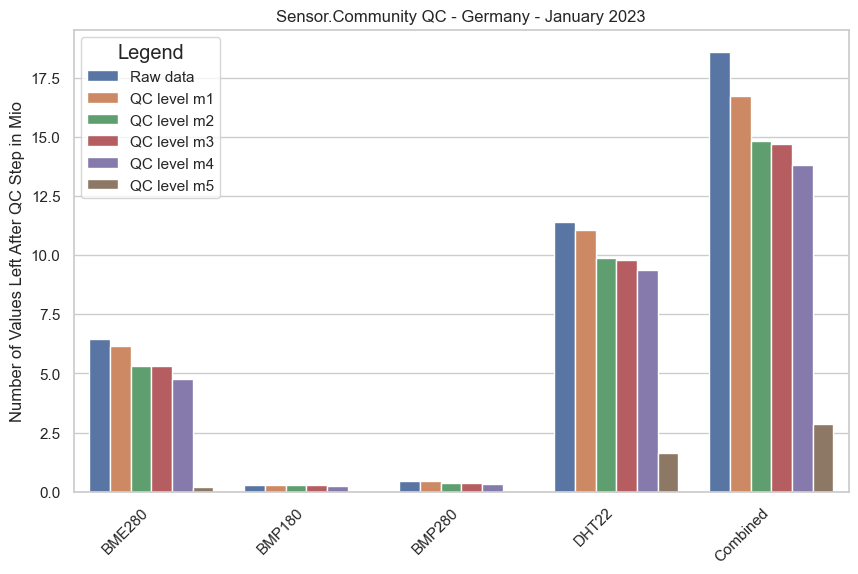
\includegraphics[width=1\textwidth]{images/sensor_community_qc_january_23.png}
    \caption{QC Results for Sensor.Community Data for Germany, January 2023}
    \label{fig:qc sensor community jan 23}
\end{figure}

\begin{figure}[ht]
    \centering
    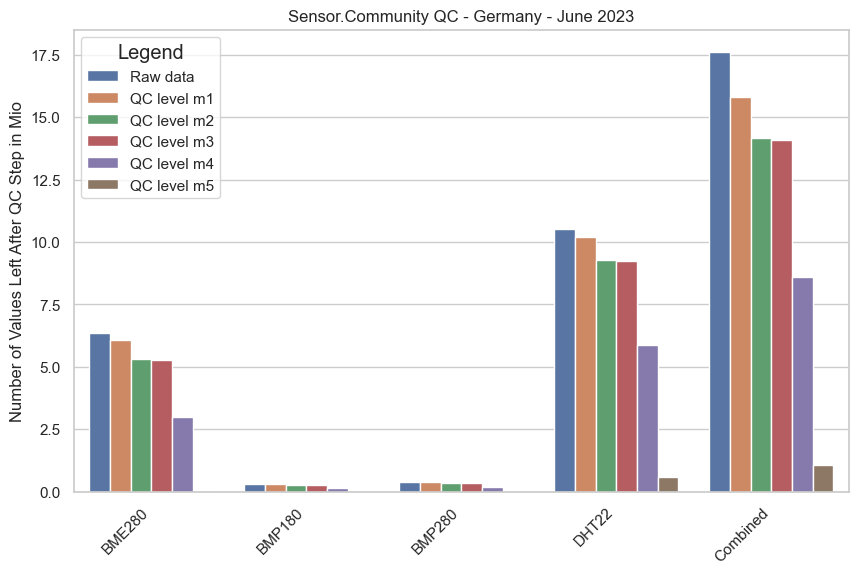
\includegraphics[width=1\textwidth]{images/sensor_community_qc_june_23.png}
    \caption{QC Results for Sensor.Community Data for Germany, June 2023}
    \label{fig:qc sensor community june 23}
\end{figure}

Here comes more data

% TODO: Update table with final data
\begin{sidewaystable}
\label{tab: qc_steps}
\caption{Quality Control Steps of CrowdQC+}
\resizebox{\textwidth}{!}{
\begin{tabular}{lllllll}
\hline
\textbf{}         & \textbf{Id} & \textbf{Name of Step}        & \textbf{Functionality}                                                                                                                                                                                                                                                        & \textbf{\% of Data} & \textbf{Num Stations} & \textbf{Num Values} \\ \hline
\textbf{Required} &             &                              &                                                                                                                                                                                                                                                                               &                                                                                    &                                                                                         &                                                                  \\
                  & m1          & Metadata Check               & \begin{tabular}[c]{@{}l@{}}Validates longitude and latitude values and removes stations with\\ identical values. Mainly aims to remove stations with default values\\ from locations from IP addresses due to improper configuration\\ by the end-user\end{tabular}           & 97.40\%                                                                            & 1077                                                                                    & 2.082.283                                                        \\
                  & m2          & Distribution Check           & \begin{tabular}[c]{@{}l@{}}Primarily targets radiative error that lead to unrealistic high ta\\ values and sensors installed indoors\end{tabular}                                                                                                                             & 86.50\%                                                                            & 1041                                                                                    & 1.849.247                                                        \\
                  & m3          & Data Validity                & \begin{tabular}[c]{@{}l@{}}Checks values of stations that did not pass m2. If more than 20\%\\ of data didn't pass the check, the station is considered to be faulty\\ and is removed\end{tabular}                                                                            & 85.20\%                                                                            & 845                                                                                     & 1.821.479                                                        \\
                  & m4          & Temporal Correlation         & \begin{tabular}[c]{@{}l@{}}Checks the temporal correlation between each station and the\\ median of all stations for a specified period of time, default 1\\ month. Targets indoor stations that have weak temporal\\ correlation to the median of all stations.\end{tabular} & 79.90\%                                                                            & 829                                                                                     & 1.708.061                                                        \\
                  & m5          & Spatial Buddy Check          & \begin{tabular}[c]{@{}l@{}}Neighbourhood-based check to identify outliers within a specific\\ area. Primarily targets radiation errors with too high ta values.\\ Defaults to radius of 3000m and 5 neighbours.\end{tabular}                                                  & 31.53\%                                                                            & 466                                                                                     & 674.004                                                          \\
\textbf{Optional} &             &                              &                                                                                                                                                                                                                                                                               &                                                                                    &                                                                                         &                                                                  \\
                  & o1          & Temporal Interpolation       & \begin{tabular}[c]{@{}l@{}}Step to interpolate missing values in the time-series of each\\ station to increase data availability\end{tabular}                                                                                                                                 & -                                                                                  & -                                                                                       & -                                                                \\
                  & o2          & Daily Validity               & Verifies robust calculations of daily values                                                                                                                                                                                                                                  & -                                                                                  & -                                                                                       & -                                                                \\
                  & o3          & Validity in Time Period      & Checks if enough values are available in a given time frame                                                                                                                                                                                                                   & -                                                                                  & -                                                                                       & -                                                                \\
                  & o4          & Correction for Time Constant & \begin{tabular}[c]{@{}l@{}}Sensors have different times that they respond to ta changes.\\ Due to Netatmo design flaws, a\\ constant correction for all stations can be applied.\end{tabular}                                                                                 & -                                                                                  & -                                                                                       & -                                                                \\ \hline
\end{tabular}}
\vspace{1ex}

{\raggedright This table shows the QC steps used in this work from the CrowdQC+ library, including the \% of data available after each step, the number of stations available and the number of values left after each step. Optional steps are currently not used. \par}
\end{sidewaystable}

\subsubsection{Handling of Moving Sensors}

Another quation arises about the ability to handle hybrid sensor network data...

\section{Feature Engineering}
\label{sec:feature_engineering}

The goal of feature engineering is to create features from the available data that can be used as input for the machine learning models. The process includes the selection of features, the extraction of features from the raw data, and the transformation of features into a format that can be used by the machine learning models.
The target feature in this work is the air temperature at 2m height. The input features are a combination of sensor readings from weather stations, sensor networks such as Sensor Community and Netatmo, as well as additonal meta data such as soil conditions, zoning plans, vegetation health, and satellite data.\\

- target variable: air temperature
- input features:
    - weather station measurements (air temperature, humidity, wind speed, wind direction, percipitation)
    - satellite data (surface temperature, surface roughness, soil temperature, land coverage indexes, sky view factor, ...)

    Need to separate between reference grade data (weather station calibrated), and low-cost sensors without placement information

- additonal goals:
    - collect mutiple datasets (many features, fine-granualar spaciotemporal)
    - enhance datasets with additonal information (soil conditions, zoning plans, vegetation health)

% TODO: Feature selection? -> remove features that are sparse etc.

Next to sensor readings captured for a given area, there are also other types of information that could be useful for ML applications. Alonso and Renard~\cite{alonso2020new} used these additional indexes to predict air temperature:

% Todo: make into table on one page
\begin{itemize}
    \item Vegetation Index
    \begin{itemize}
        \item Normalized Difference Vegetation Index (NDVI)
        \item Soil Adjusted Vegetation Index (SAVI)
        \item Enhanced Vegetation Index (EVI)
        \item Tasseled Cap Transformation greenness (GVI)
        \item Density of low vegetation
        \item Density of medium vegetation
        \item Density of high vegetation
    \end{itemize}
    \item Water Presence Index
    \begin{itemize}
        \item Modified Normalized Difference Water Index (MNDWI)
        \item Normalized Difference Water Index (NDWI)
    \end{itemize}
    \item Moisture Index
    \begin{itemize}
        \item Tasseled cap Transformation Wetness
        \item Normalized Difference Moisture Index (NDMI)
    \end{itemize}
    \item Bare Soil Index
    \begin{itemize}
        \item Normalized Difference Bareness Index (NDBaI)
        \item Bare Soil Index (BI)
        \item Enahnced Build-Up and Bareness Index (EBBI)
        \item Density of bare soil
    \end{itemize}
    \item Radiation Index
    \begin{itemize}
        \item Spectral radiance
        \item Emissivity
        \item Tasseled Cap Transformation Brightness
    \end{itemize}
    \item Building Index
    \begin{itemize}
        \item Normalized Difference Build-Up Index (NDBI)
        \item Urban Index (UI)
        \item Index-based Build-Up Index (IBI)
        \item Building Density
    \end{itemize}
    \item Topographic
    \begin{itemize}
        \item Slope (°)
        \item Exposure
        \item Curvature
    \end{itemize}
    \item Urban morphology
    \begin{itemize}
        \item Sky View Factor
        \item Standard Deviation (STD) of Building Height (building height variation)
    \end{itemize}
    \item Land use
    \begin{itemize}
        \item Distance to railway tracks
        \item Distance to points of tourist interest
        \item Distance to subway entrances
        \item Distances to fountains
        \item Water area
    \end{itemize}
\end{itemize}

These types of data can be sourced either directly via satellites like LiDAR or Landsat 8, or via geoportals that publish such data, like the State Office for Geoinformation and Surveying Hamburg~\footnote{\url{https://geoportal-hamburg.de/geo-online/}} on a regional basis or the EU Inspire Geoportal~\footnote{\url{https://inspire-geoportal.ec.europa.eu/}} on a continental basis.

ref to google earth engine~\cite{gorelick2017google}

Features:
- completed:
    - ndvi, evi (modis) -> 500m, 16 days
- todo:
    - lai, nb


Hyperlocal Mapping in Oslo:
Red Landsat 7, 8 and Sentinel 2 Open source L: 30 m, S: 10 m Green Blue Near infrared Short-wave infrared 1 L: 30 m, S: 20 m Short-wave infrared 2 NDVI L: 30 m, S: 10 m IBI L: 30 m, S: 20 m Land surface temperature Landsat 7, 8 30 m Elevation above sea STRM 30 m Terrain aspect Terrain slope Terrain ruggedness CHM LiDAR Closed source 1m CHM slope CHM aspect CHM shadow/SVI Building height LiDAR + building footprint Building height sd 1–4m Building height sd 4–20 m Building height sd 20–100 m Fractional tree cover LiDAR + orthophoto Tree height Distance to coast Global water occurrence Open source 30 m Distance to fresh water